\section{User Study}

\begin{figure}[tp]
    \centering
    \setlength{\belowcaptionskip}{-25pt}
    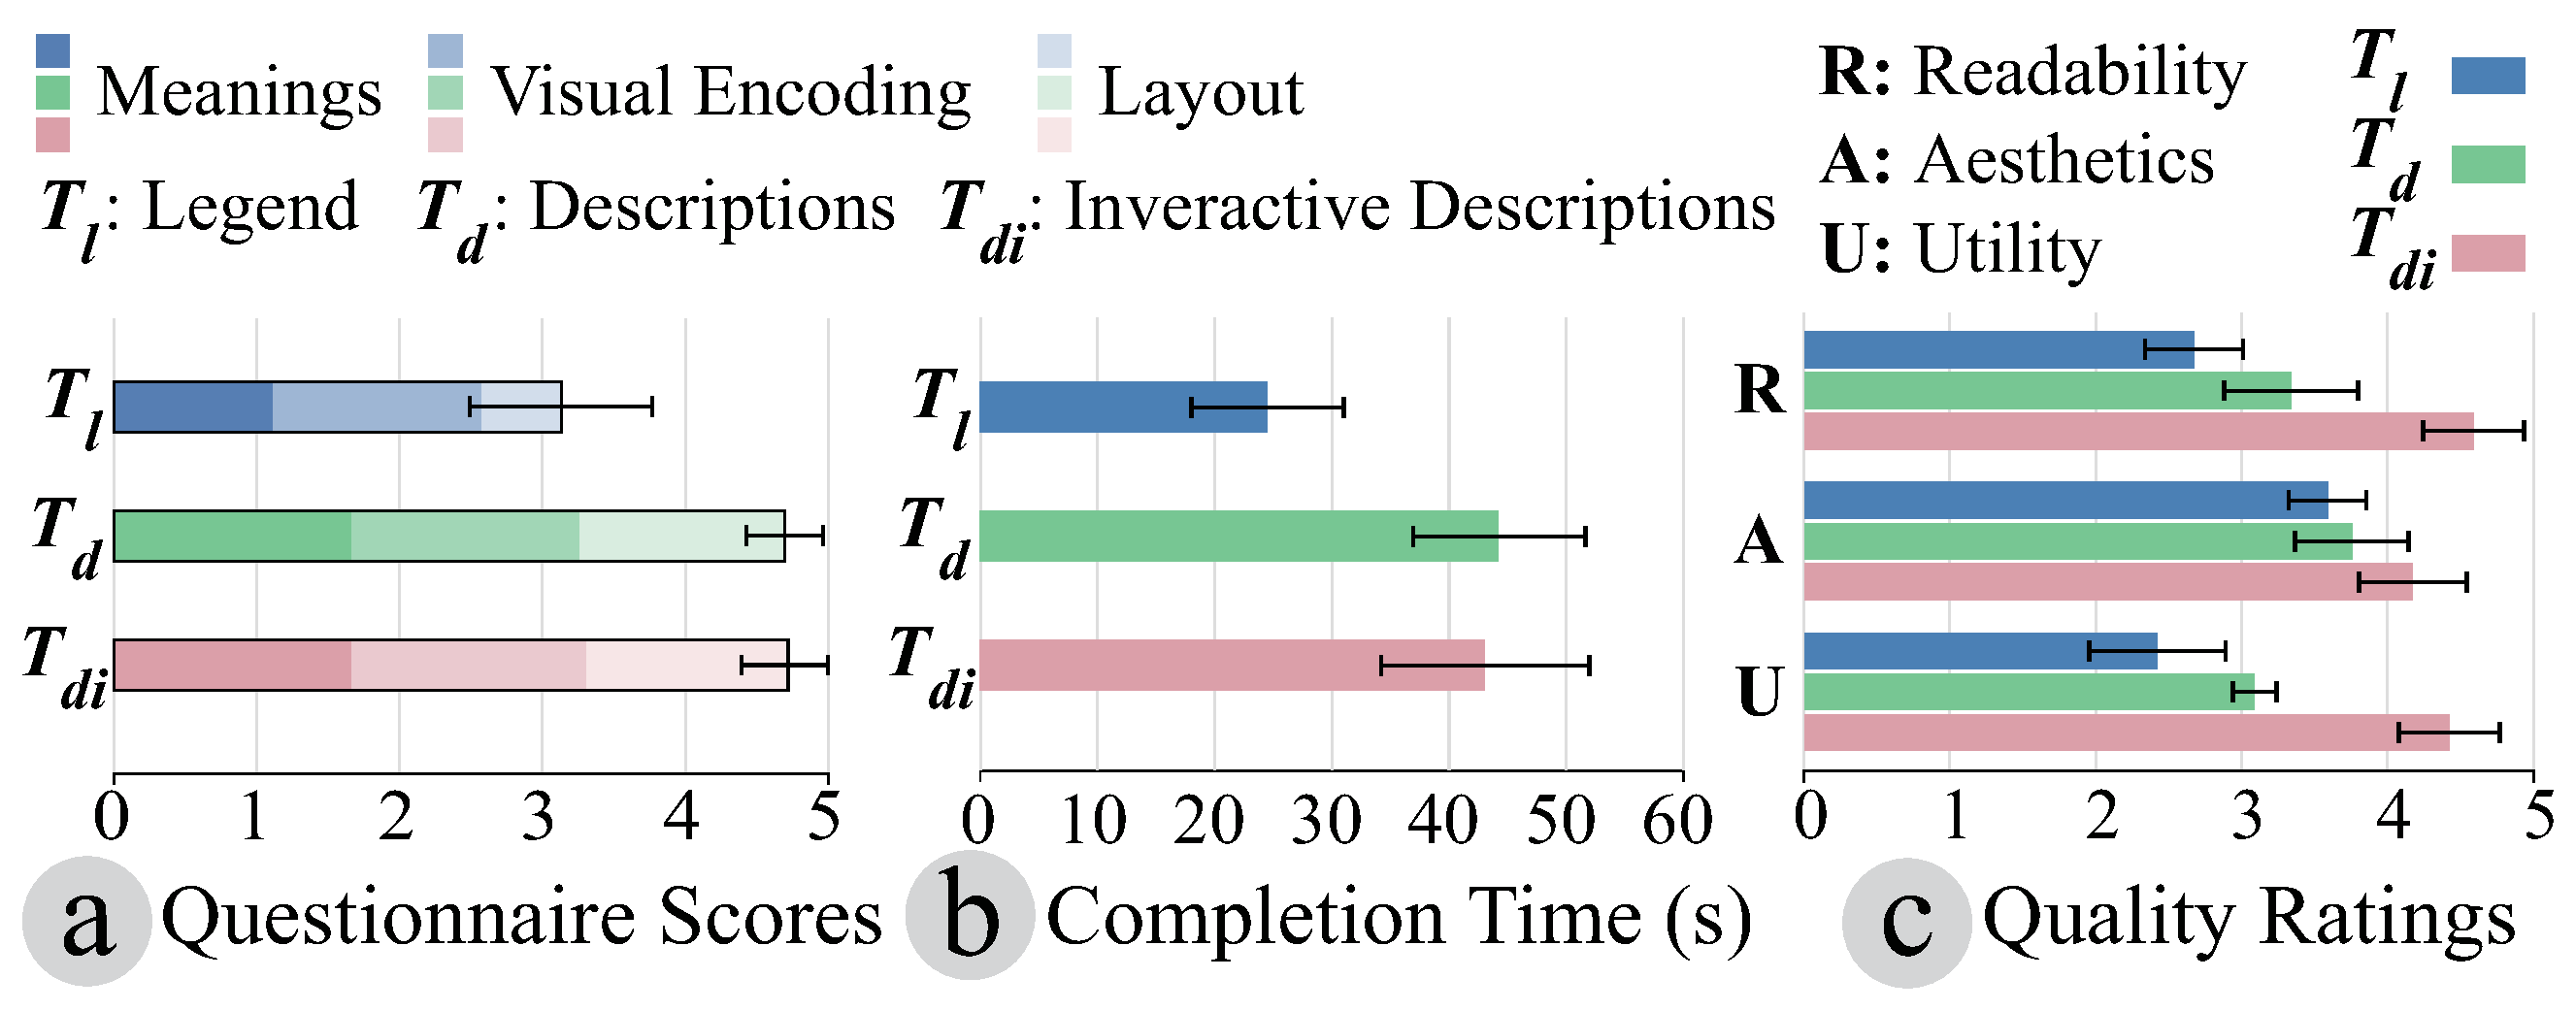
\includegraphics[width=1\columnwidth]{figures/UserStudy.eps}
    \caption{The result of our user study with the mean values of $95\%$ confidence intervals. (a) The questionnaire score distributions of three techniques, (b) the average completion time distributions of three techniques, and (c) the distribution of ratings of different metrics of our interactive descriptions. }
    \label{fig:UserStudy}
\end{figure}


We conducted a qualitative user study to assess the effectiveness of~\ApproachName. The study aimed to evaluate whether our approach can enhance the comprehensibility of node-link diagrams. This study chooses one of the most classic scheme -- the legend, as our baseline. We evaluated our approach's effect on comprehensibility enhancement by comparing the effect of the legend, our generated descriptions, and descriptions without interactions.


\textbf{Participants.}
We recruited 12 participants in the study (P1-P12; 4 males; aged: 22-26 ($\mu$=23.58, $\sigma$=1.32)). All participants are students or researchers from the Computer Science department, three of them majored in Visualization with professional experience in analyzing node-like diagrams, and the others have the basic visualization knowledge by taking the relevant courses. The scale of expert participants is consistent with similar graph visualization research~\cite{DBLP:journals/tvcg/BehrischSP20, DBLP:journals/tvcg/YoghourdjianDKM18}. Each participant received a gift card worth \$15 at the beginning, independent of their performance.


\textbf{Task. }
We chose the three node-link diagrams used in Section~\ref{sec:casestudy} as our test material. We prepared three types of descriptions: $T_l$ is the legend, which serves as the control group, $T_d$ is our descriptions without interaction, and $T_{di}$ is our interactive descriptions. For the legend, there is no standard design to convey information about the layout type. Our legends design only displays the layout type with text (``topology'') and axes (attributes). For each diagram, there will be 
several detailed descriptions samples (ten in case 1, eight in case 2, and eight in case 3) with different types of information (link conditions, visual encodings, and layout type).  To sum up, a complete task contains: 3 \emph{descriptions conditions} $\times (10+8+8)$ \emph{samples} = 78 trials. 

\textbf{Procedure. }
The study began with an introduction (three minutes) of the study purpose, study materials and the study tasks. During the practice phase (five minutes), participants were equipped with a mouse to explore node-link diagrams, legends, and descriptions freely.

After the training, participants started the formal tasks, which lasted for around one hour. We recorded the exploration time and successfulness of each trial. Each trial ended with a post-study questionnaire (one minute) to evaluate the understanding degree of users, which reflects the comprehensibility of our approaches. The questions for the three diagrams are consistent with the three parts of information summarized in Section~\ref{sec:pilotstudy}. 
The total score of one participant was scaled to a five-point score.

After each task, participants were asked to rate four five-point Likert scale questionnaires regarding readability, aesthetics, and utility. Besides, they were encouraged to give suggestions for our techniques.

\subsection{Results, Findings and Lesson Learned}
We consider that the study assessed the system qualitatively rather than quantitatively due to the small sample size. 


\textbf{Comprehensibility}.
The higher the score, the better comprehensibility of node-link diagrams. Overall, the results of $T_d$ ($\mu$=4.72, $\sigma$=.94), $T_{di}$ ($\mu$=4.70, $\sigma$=.79)) and $T_l$ ($\mu$=3.13, $\sigma$=1.86) are shown in Figure~\ref{fig:UserStudy}a. For non-parametric statistical significance test results, the Friedman test suggests significance among three techniques ($p<.05$), and the Wilcoxon Signed-Rank test suggests $T_l$ gets lower scores than both $T_d$ and $T_{di}$ ($p<.05$). No significance is suggested between $T_d$ and $T_{di}$ ($p=.72$). 
We repeated the two tests on the scores of different description types (link conditions, visual encodings, and layout type), and found that $T_d$ and $T_{di}$ were significantly better than $T_l$ while no significance was detected between $T_d$ and $T_{di}$.
The results reported that our two techniques enhanced the comprehensibility of node-link diagrams compared with the legend.
Most of the participants commended our descriptions: \textit{``I do not need to speculate information when viewing descriptions. They are comprehensive and precise.''} 

\begin{itemize}[noitemsep,topsep=0pt,parsep=0pt,partopsep=0pt, leftmargin=20pt]
    \item {\bf Finding 1}: 
    The comprehensibility improvement made by our descriptions mainly comes from the completeness of needed information. The hover-then-highlight interaction helps little to the comprehensibility.
    \item {\bf Lesson Learned 1}: 
    To augment comprehensibility, we can explore other interaction methods and develop more comprehensive descriptions.
\end{itemize}

{\bf Efficiency.} Users reported that the relatively high information granularity of our descriptions makes them spend more time on exploration and relevant information selection. And the analysis on completing time supports their report. 
By employing the two non-parametric statistical significance tests, we find the time of using $T_d$ ($\mu$=44.25, $\sigma$=11.01) and $T_{di}$ ($\mu$=43.10, $\sigma$=13.40) is significantly higher ($p$<.05) than $T_l$ ($\mu$=24.51, $\sigma$=9.81).
We also find there is no significant difference between $T_d$ and $T_{di}$ ($p=.58$). Our interaction has little impact on the exploration time of the task.

\begin{itemize}[noitemsep,topsep=0pt,parsep=0pt,partopsep=0pt, leftmargin=20pt]
    \item {\bf Finding 2}: Exhaustive description costs people more time to explore and select information.
    \item {\bf Lesson Learned 2}: We need to balance the comprehensiveness and conciseness of information. We can highlight some partial information on the descriptions according to usage scenarios and user preferences.
\end{itemize}


\textbf{Utility}.
We found that our participants rated the utility of $T_{di}$ ($\mu$=4.42, $\sigma$=.67) significantly higher than $T_d$ ($\mu$=3.08, $\sigma$=.29), and the utility of $T_d$ is also significantly higher ($p$<.05) than $T_l$ ($\mu$=2.42, $\sigma$=.90).
It means our participants prefer interactive descriptions.
P10 said the interaction attracted his interest to read the description.
P3 mentioned that the spatial relationship between descriptions and the node-link diagram affected his information searching and mapping.
Two participants (P5 and P11) suggested generating tooltips to show the information of each data entity.

\begin{itemize}[noitemsep,topsep=0pt,parsep=0pt,partopsep=0pt, leftmargin=20pt]
    \item {\bf Finding 3}: The distance between descriptions to visualization affects the utility.
    \item {\bf Lesson Learned 3}: We need to consider the spatial relationship between visualization and descriptions. And the tooltip might be an alternative to the current hover-then-highlight interaction.
\end{itemize}

\textbf{Aesthetics}.
The Friedman significance test suggested there is no significance among our descriptions and the legend ($p$=.08).
P1 commented that \textit{``Text colors of descriptions are a little complex.''} She suggested reducing the design complexity by using fewer fonts and colors to highlight essential information.

\begin{itemize}[noitemsep,topsep=0pt,parsep=0pt,partopsep=0pt, leftmargin=20pt]
    \item {\bf Finding 4}: Over-considering the information does not improve readability, but also increases cognitive load for users.
    \item {\bf Lesson Learned 4}: we should rank the importance of different information, and only highlight the most important information.
\end{itemize}

\textbf{Readability}.
Two significance tests suggested that $T_{di}$ ($\mu$=4.50, $\sigma$=.80) is more readable than $T_d$ ($\mu$=3.33, $\sigma$=.89) and $T_l$ ($\mu$=2.67, $\sigma$=.65). And $T_d$ makes no difference to $T_l$.
Although our interaction helps to improve the comprehensibility a bit, it improves the readability of our descriptions.
Most of our participants praised our interaction design, such as \textit{``The interaction locates the target visual elements for me to track and solve questions.''} 
P10, who gave a low score for the readability, commented that descriptions of visual encodings were too trivial for him to find the required information. 
He suggested replacing trivial and repetitive text with symbols, such as icons and arrows.
% Another participant suggested us to generate descriptions with multilingual versions. It can help non-native English users to understand node-link diagrams.
 

\begin{itemize}[noitemsep,topsep=0pt,parsep=0pt,partopsep=0pt, leftmargin=20pt]
    \item {\bf Finding 5}: Trivial and repetitive templates affect the readability of descriptions.
    \item {\bf Lesson Learned 5}: We should explore more organizing forms of descriptions. And replacing repetitive texts with icons such as arrows and emojis may improve the readability.
\end{itemize}

